\chapter{Design patterns[2]}\label{Chapter:Design patterns}
I denne iteration af CDIO-projektet \cite{CDIOdel2} har en del af udviklernes opmærksomhed været rettet mod "godt design" på kode-niveau. Diskutioner og beslutninger er hovedsageligt foregået/taget på baggrund af første halvdel af GRASP-principperne som de er præsenteret til og med kapitel 24 i \cite{umlbook}. Dette omfatter følgende design patterns/principper: 

\begin{itemize}
	\item High Cohesion    
	\item Low Coupling
	\item Information Expert
	\item Creator
	\item Controller
\end{itemize}





Hvert af principperne gennemgåes yderligere i \vref{Chapter:Design patterns:Anvendelse}.

Til grund for al OO-udvikling ligger principperne \dpattern{High Cohesion} og \dpattern{Low Coupling}. Dette skyldes at vi på denne måde "nemt" får grupperet kodedele der hører logisk sammen, altså OOD. Dette gør vi, fordi det resulterer i et mere overskueligt og lettere vedligeholdt system.
\fxnote{OO forkortelse anvendt uden forklarende tekst inden.} 
 
\section{Anvendelse}\label{Chapter:Design patterns:Anvendelse}
%Jeg har anvendt \textit{} lidt løst. Jeg er lidt i tvivl om hvad jeg skal gøre når jeg skal %henvise til design patterns og instansvariabler. De får indtil videre samme behandling.

\subsection{High Cohesion}\label{Chapter:Design patterns:Anvendelse:High Cohesion}
Da \dpattern{High Cohesion} nærmere er et overordnet princip end et egentligt design pattern er det også anvendt gennem hele systemets design. \dpattern{High Cohesion} handler om at samle dele af et program, der logisk har tætte relationer. På denne måde opnår man, at hver klasse kun tager sig af en type operationer. Dermed bliver hele programmets struktur lettere at overskue. I \textit{matador} systemet har hver klasse sin specifikke opgave. \klasse{Die} er kun terning og indeholder således kun metoder der hænger tæt sammen med det "at være terning". \klasse{MatadorRafleBaeger} indeholder også kun metoder der har med et raflebægers funktion at gøre. Raflebægeret har tætte relationer med terningerne i det, men de er hver deres entitet og er således opdelt i hver deres klasse. Dog har raflebægeret kendskab til terningerne hvilket uddybes mere i \vref{Chapter:Design patterns:Anvendelse:Creator}.       

\subsection{Low Coupling}\label{Chapter:Design patterns:Anvendelse:Low Coupling}
I forlængelse af og samspil med \dpattern{High Cohesion} følger \dpattern{Low Coupling}. Hvor \dpattern{High Cohesion} handler om samling i vertikaler, siger \dpattern{Low Coupling} i modsætning noget om programmets horisontale struktur. Altså hvor og hvordan de enkelte vertikaler "hænger" sammen. Her er fokus bl.a. på hvem der skal have kendskab til hvem. Der er fx ingen grund til at lade \klasse{Die} have kendskab til \klasse{matadorRafleBaeger}. En terning bruges af andre og der er dermed grundlag for at andre skal kende terningen, men ikke omvendt. Ved at lade disse ideer gennemsyre et helt system opnås \dpattern{Low Coupling} nemmere og således bliver systemet også lettere at vedligeholde, da hver vertikal har mindst mulig indflydelse på andre vertikaler. Et andet eksempel på \dpattern{Low Coupling} er \klasse{BoundaryToPlayer}. Denne klasse overholder \dpattern{High Cohesion} ved kun at have med præsentation af information i konsollen at gøre. Samtidig overholdes også \dpattern{Low Coupling} da den ikke har kendskab til andet end de objekter den henter information ud af. Man kan, med rette, argumentere for, at der brydes med \dpattern{Low Coupling} ved, at overføre objekter istedet for kun at overføre den specifikke data \klasse{BoundaryToPlayer} skal bruge. Der er taget et valg om at gå fra det ene design til det andet for \textit{matador} systemets vedkommende. Valget skyldes, at det at overføre data gennem flere klasser giver mange redundante metoder gennem systemet. Derfor, hvis et objekt har mere end en attribut der skal overføres til \klasse{BoundaryToPlayer} kan der spares en del kode ved, at placere logikken til at hente informationerne ud, i \klasse{BoundaryToPlayer}. I \vref{fig:highCoupling} og \vref{fig:lowCoupling} ses henholdsvis High Coupling, Low Cohesion og Low Coupling, High Cohesion skitseret.\fxnote{Syntes ordet \enquote{vertikaler} lyder lidt mærkeligt}

\begin{figure}
\caption{High Coupling og Low Cohesion}
\label{fig:highCoupling}
\centering
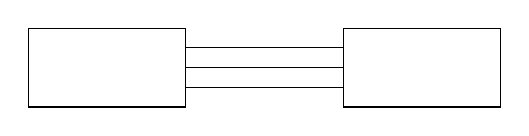
\begin{tikzpicture}
	\draw (-4,0) rectangle (-2,1);
	\draw (0,0) rectangle (2,1);
	\draw (-2,0.5) -- (0,0.5);
	\draw (-2,0.75) -- (0,0.75);
	\draw (-2,0.25) -- (0,0.25);
\end{tikzpicture}
\end{figure}

\begin{figure}
\caption{Low Coupling og High Cohesion}
\label{fig:lowCoupling}
\centering
\begin{tikzpicture}
	\draw (-3,0) rectangle (-2,2);
	\draw (0,0) rectangle (1,2);
	\draw (-2,1) -- (0,1);
\end{tikzpicture}
\end{figure}

\subsection{Information Expert}\label{Chapter:Design patterns:Anvendelse:Information Expert}
Dette pattern hænger meget tæt sammen med, og fremkommer af, begrebet "responsibility assignment". Det kan tolkes som "den der ved det, formidler det!". Indehaveren af en given information bliver altså tildelt ansvaret for også at videreformidle den. Et godt eksempel på anvendelse af \dpattern{Information Expert} kan findes i \klasse{Die}. Her er det oplagt at instanser af \klasse{Die} er eksperter på egne \textit{facevalues}. Dermed består "responsibility assignment", for \klasse{Die}, i metoder som \metode{getFaceValue} og \metode{rollDie}. 

\subsection{Creator}\label{Chapter:Design patterns:Anvendelse:Creator}
Navnet fortæller meget godt hvad dette pattern gør. Nemlig at skabe. \dpattern{Creator} pattern anvendes for at finde ud af hvilken klasse der skal skal skabe instanser af andre klasser. Iflg. \dpattern{Creator} skal en klasse A, instansiere en anden klasse B, hvis A: omslutter, aggregerer, optager, tæt bruger eller har initialiseringsdata for B \cite{umlbook}. Således er det et meget benyttet pattern simplethen fordi dets brug ligger i kernen af OO udvikling. Et eksempel på en situation hvor dette pattern bør anvendes findes i \klasse{matadorRafleBaeger}. Her bør Creator benyttes til instansiering af \klasse{Die} fordi netop entiteten raflebæger indeholder og bruger terninger. 

\subsection{Controller}\label{Chapter:Design patterns:Anvendelse:Controller}
Brugen af \dpattern{Controller} pattern kan udmønte sig i flere forskellige løsninger på samme problem. Dette skyldes at implementationen af \dpattern{Controller} hænger tæt sammen med det resterende programs udformning, størrelse og formål. I denne iteration af CDIO-projektet er noget af spillets logik og "styringen" af spillets flow lagt i samme \dpattern{Controller}/logik klasse, \klasse{Game}. Denne løsning kan fx andvendes, som her, til mindre systemer, hvor en opdeling af klasserne til håndtering af logik og flow synes overflødig pga. systemets relativt lille og overskuelige størrelse. I denne iteration af projektet er det blevet valgt at følge netop denne model. Resultatet er en klasse \klasse{Game} der er en smule "bloated" og med en smule mindre samhørighed (\vref{Chapter:Design patterns:Anvendelse:High Cohesion}) samt lidt højere kobling (\vref{Chapter:Design patterns:Anvendelse:Low Coupling}) sammenlignet med resten af systemets klasser. Det understreges, at denne model er et særtilfælde og ikke tydeligt understøtter gængse OO-principper. Dens anvendelse kan dog forsvares med systemts relativt lille kompleksitet. Det nævnes at \cite{umlbook} behandler dette nøjagtige eksempel i kap. 17.

De andre muligheder for \dpattern{Controller} som præsenteret i \cite{umlbook} er tilfælde for systemet enten opererer i en lukket enhed (tlf. og bank er brugt som eksempler) og den anden, og for dette projekt relevante, tager udgangspunkt i bce/mvc-modellerne. Denne løsningsmodel har til formål at adskille kommunikation og logik. Her ved at lade \klasse{Game} blive opdelt i 2 klasser. Heraf vil den ene fungere som en "ren" \dpattern{Controller} og den anden som en "ren" entity-klasse. Ved brug af denne model ligner systemets design i højere grad bce-modellen og \dpattern{Controller} klassens "ansvarsområde"  ville således kunne overføres direkte fra Use Case Modellen.        




